\documentclass[border=8pt]{standalone}
\usepackage{tikz,amsmath,amssymb,bm}
\usetikzlibrary{arrows.meta,calc,angles,quotes,decorations.markings}
\begin{document}
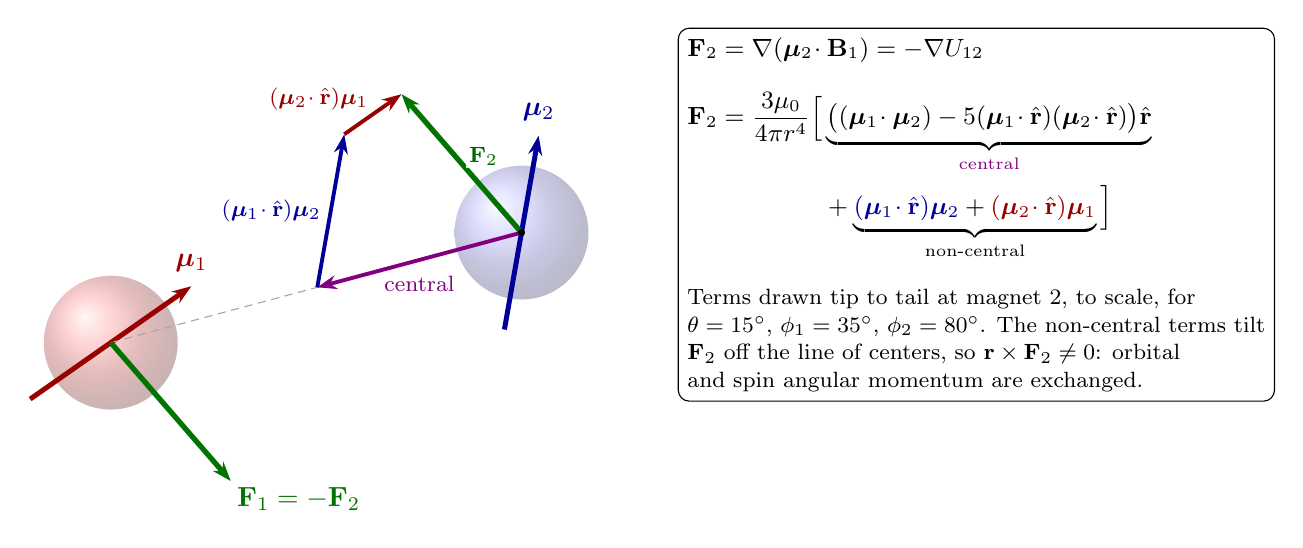
\begin{tikzpicture}[>={Stealth[length=7pt,width=5pt]},
  mom/.style={->,line width=1.8pt}, vec/.style={->,line width=1.1pt},
  aux/.style={densely dashed,gray!70},
  lbl/.style={fill=white,fill opacity=0.85,text opacity=1,inner sep=1pt,font=\footnotesize}]
\coordinate (P1) at (0,0);\coordinate (P2) at (5.2160,1.3976);
\shade[ball color=red!65!white,opacity=0.35] (P1) circle (0.85);
\shade[ball color=blue!45!white,opacity=0.35] (P2) circle (0.85);
\draw[mom,red!60!black] (P1) ++(215:1.25) -- ++(35:2.5) node[above=1pt] {$\bm\mu_1$};
\draw[mom,blue!60!black] (P2) ++(260:1.25) -- ++(80:2.5) node[above=1pt] {$\bm\mu_2$};

\draw[aux] (P1) -- (P2);
\draw[vec,violet,line width=1.4pt] (5.2160,1.3976) -- (2.6225,0.7027) node[midway,below=4pt,lbl,text=violet] {central};
\draw[vec,blue!60!black,line width=1.4pt] (2.6225,0.7027) -- (2.9652,2.6461) node[midway,left=2pt,lbl,text=blue!60!black] {$(\bm\mu_1\!\cdot\hat{\mathbf r})\bm\mu_2$};
\draw[vec,red!60!black,line width=1.4pt] (2.9652,2.6461) -- (3.6922,3.1551) node[midway,above left=0pt,lbl,text=red!60!black] {$(\bm\mu_2\!\cdot\hat{\mathbf r})\bm\mu_1$};
\draw[vec,green!45!black,line width=1.9pt] (5.2160,1.3976) -- (3.6922,3.1551) node[pos=0.55,right=3pt,lbl,text=green!40!black] {$\mathbf F_2$};
\draw[vec,green!45!black,line width=1.9pt] (P1) -- ++(1.5238,-1.7575) node[below right=-2pt] {$\mathbf F_1=-\mathbf F_2$};
\fill (P2) circle (1.3pt);
\node[draw,rounded corners,fill=white,align=left,anchor=north west,font=\small] at (7.2,4.0) {%
 $\displaystyle \mathbf F_2=\nabla(\bm\mu_2\!\cdot\mathbf B_1)=-\nabla U_{12}$\\[10pt]
 $\displaystyle \mathbf F_2=\frac{3\mu_0}{4\pi r^4}\Big[\underbrace{\big((\bm\mu_1\!\cdot\bm\mu_2)-5(\bm\mu_1\!\cdot\hat{\mathbf r})(\bm\mu_2\!\cdot\hat{\mathbf r})\big)\hat{\mathbf r}}_{\color{violet}\text{central}}$\\[4pt]
 $\displaystyle \hphantom{\mathbf F_2=\frac{3\mu_0}{4\pi r^4}\Big[}+\underbrace{{\color{blue!60!black}(\bm\mu_1\!\cdot\hat{\mathbf r})\bm\mu_2}+{\color{red!60!black}(\bm\mu_2\!\cdot\hat{\mathbf r})\bm\mu_1}}_{\text{non-central}}\Big]$\\[10pt]
 \footnotesize Terms drawn tip to tail at magnet 2, to scale, for\\[-1pt]
 \footnotesize $\theta=15^\circ$, $\phi_1=35^\circ$, $\phi_2=80^\circ$. The non-central terms tilt\\[-1pt]
 \footnotesize $\mathbf F_2$ off the line of centers, so $\mathbf r\times\mathbf F_2\neq 0$: orbital\\[-1pt]
 \footnotesize and spin angular momentum are exchanged.};
\end{tikzpicture}
\end{document}
